\section{Future Scope: Local LLMs and Multi-Purpose Transformer Silicon}
\label{sec:future}

RouteVoice combines full-recognizer RTL with one separately routed projection engine and separately generated index banks. This section sets out what the same techniques imply for local language models and for silicon that serves more than one transformer. Unlike the rest of the paper, these are projections, not measurements.

\subsection{From recognizer to voice assistant}
A useful local voice device chains speech-to-text, a small language model, and text-to-speech. Transformer-based choices for these stages share dense projections, attention and normalization, but their frontends, state, operators and scheduling can differ.

The projection engine here is model-agnostic below the index fabric. It consumes a stream of signed activations and a fixed table of 4-bit selections, and emits FP32 results. A second model would also require compatible shapes and numerics, new books and metadata, control and state planning, and validation of unsupported operators. Reuse of this projection mechanism is a possibility, not demonstrated multi-model compatibility.

Mutable state is an additional scaling constraint alongside fixed-weight storage, arithmetic and integration. A recognizer's mutable state is its audio window and decoder cache. An autoregressive LLM adds a key/value cache that grows with context, which belongs in SRAM or external DRAM, never in metal.
For scale, a 0.5\,B-parameter LM such as Qwen2.5-0.5B~\cite{qwen2024qwen25,qwen05config} (24 layers, two key/value heads of dimension 64) keeps 6,144 key/value values per token. At 8 bits, a 2,048-token context needs about \SI{12.6}{MB}, roughly twelve times all of RouteVoice's mutable state (8.17\,Mbit).

\subsection{Hardwired weights at larger scale}
Fixed-index storage has a clear scaling trade:
\begin{itemize}
\item \textbf{Benefits:} fixed coefficients need no off-chip weight transfers; local index/book readout still costs energy, and mutable state can still require off-chip bandwidth. This does not establish a security property.
\item \textbf{Cost:} a mask set per model.
\end{itemize}
Commercial hardwired-LLM efforts~\cite{taalas2026hc1} accept that cost at the frontier for throughput.

Our results suggest a complementary point at the low end, and they let us size it.

\paragraph{Throughput.} A dense decoder-only LM of $N$ parameters needs about $N$ multiply-accumulates per generated token. One of our engines sustains \SI{0.66}{GMAC/s} at \SI{6.67}{MHz}. Ignoring attention, state transfers, control, utilization and inter-engine communication gives a MAC-only upper bound of about 1.3 tokens/s per engine, or 13 for ten ideally utilized engines. These are not measured generation rates or demonstrated voice-assistant latency.

\paragraph{Area.} Index area alone is already a major constraint; this calculation excludes compute and mutable state. At our measured \SI{5.54}{\micro m^2} per selection, 0.5\,B selections need about \SI{2800}{mm^2} at \SI{180}{nm}, several reticles.

\paragraph{Node scaling.} Ideal area scaling to \SI{28}{nm} is $(180/28)^2\approx41\times$, which would bring the same banks to roughly \SI{70}{mm^2}. Peripheral circuits scale worse than this, so the figure is an optimistic bound. \Cref{fig:scaling} plots the measured points and an assumed 20--40$\times$ band, without a physical port validating either endpoint.

\begin{figure*}[t]
\centering
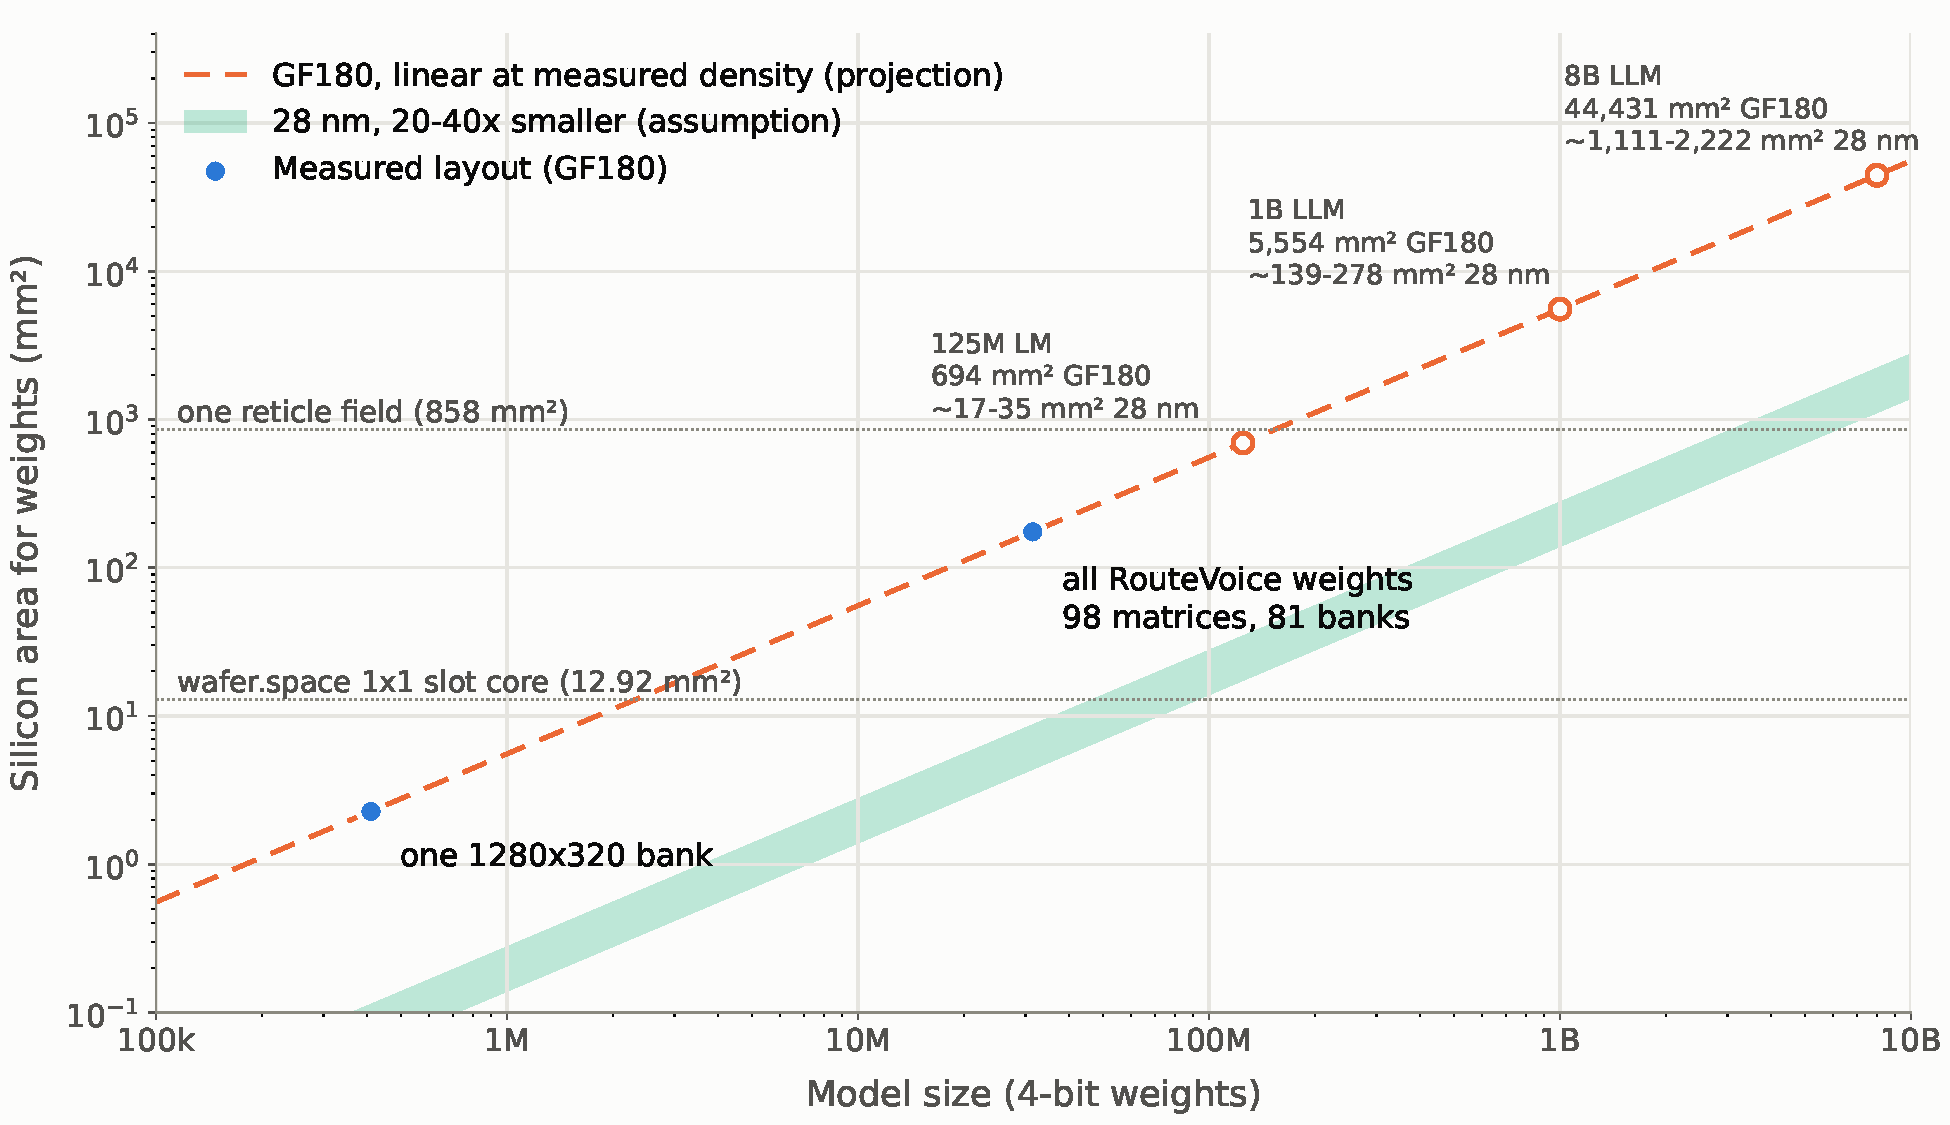
\includegraphics[width=0.8\textwidth]{figures/scaling-area.pdf}
\caption{Weight-array area against model size. Filled points are measured GF180 layout: one $1280\times320$ bank (\SI{2.27}{mm^2}) and all 98 RouteVoice matrices (\num{31457280} four-bit weights, \SI{174.7}{mm^2}, i.e.\ \SI{5.55}{\micro m^2} per weight including readout). The dashed line extends that density linearly; the shaded band assumes a 20--40$\times$ area reduction at \SI{28}{nm}. Both are projections, not measurements. Weights only: compute engines, activation and KV memory, and I/O are excluded.}
\label{fig:scaling}
\end{figure*}

\paragraph{Where this leaves the low end.} This work lays out the fixed indices for a tens-of-millions-parameter speech model on a mature node. It does not establish a complete recognizer fit, yield or cost. A sub-billion-parameter LM would require substantial density improvement before even its fixed indices approach a practical single-die area; affordability also depends on integration and manufacturing economics.

\subsection{Making hardwired silicon multi-purpose}
Hardwiring trades flexibility for efficiency. Several mechanisms can recover flexibility without returning to fully programmable weights:
\begin{enumerate}
\item \textbf{Mutable codebooks over fixed indices.} The 4-bit indices are fixed; the 16-entry books (\SI{4.9}{MB} for the services we converted, about half the index bytes) could instead live in SRAM. Then one die could be re-tuned after fabrication: recalibrated, rescaled, or fine-tuned within the span its fixed indices allow. At open-SRAM density that costs far more area than the books do as ROM, so it suits a model family whose indices are shared and whose books differ. Whether book-only fine-tuning recovers useful accuracy is an experiment we have not run.
\item \textbf{Low-rank adapters in SRAM.} A fixed base model plus small SRAM-resident adapters (LoRA-style) on selected projections supports task or speaker adaptation. The existing 160-SRAM bridge tests memory protocols only; it does not implement or validate LoRA arithmetic or adaptation.
\item \textbf{Shared backbones.} Distilling several tasks onto one shared encoder lets one fixed fabric serve many heads: transcription, keyword spotting, intent, language identification. Only the small task heads stay mutable.
\item \textbf{Family dies.} A mask set can hold several small models whose index fabrics share one engine and I/O ring, selected at run time. Area grows linearly in model bytes, but NRE is paid once.
\end{enumerate}

\subsection{Economics}
The economic case depends on volume, yield, packaging and model lifetime. Open-PDK shuttles~\cite{waferspace} provide a possible route to small test structures, but the current \SI{22.84}{mm^2} engine already exceeds an approximately \SI{20}{mm^2} slot before adding its array and I/O. The two proposed \SI{725}{mm^2} dies are a different manufacturing scale. We have no verified quotation for a complete recognizer and make no affordability claim.

This project documents an AI-assisted design process; it does not measure a causal speedup over a controlled alternative. Potential applications include appliance voice control, wearables and industrial sensors whose model can remain fixed, subject to resolving the energy, timing, quality and integration limits above.
